% ---------------------------------------------------------------
% ---------------------------------------------------------------
% This template was developed for the working paper series of 
% the Interdisciplinary Laboratory of Computational Social Science (iLCSS)
% at the University of Maryland, College Park

% The template was built based on  the PNAS Latex model. 

% Adjustments were made by Tiago Ventura, Ph.D. Student in Political Science at UMD, 
% and researcher at the iLCSS.

\documentclass[9pt,twocolumn,twoside]{ilcss}




\templatetype{ilcssworkingpaper} % Choose template 

\title{Working Paper series Interdisciplinary Laboratory of Computational Social Science (iLCSS)}	

% Use letters for affiliations, numbers to show equal authorship (if applicable) and to indicate the corresponding author
\author[a,c,1]{Author One}
\author[b,1,2]{Author Two} 
\author[a]{Author Three}

\affil[a]{Affiliation One}
\affil[b]{Affiliation Two}
\affil[c]{Affiliation Three}

% Please give the surname of the lead author for the running footer
\leadauthor{Lead author last name} 

% Please add here a significance statement to explain the relevance of your work
\significancestatement{Authors must submit a 120-word maximum statement about the significance of their research paper written at a level understandable to an undergraduate educated scientist outside their field of speciality. The primary goal of the Significance Statement is to explain the relevance of the work in broad context to a broad readership. The Significance Statement appears in the paper itself and is required for all research papers.}

% Please include corresponding author, author contribution and author declaration information
\authorcontributions{Please provide details of author contributions here.}
\authordeclaration{Please declare any conflict of interest here.}
\equalauthors{\textsuperscript{1}A.O.(Author One) and A.T. (Author Two) contributed equally to this work (remove if not applicable).}
\correspondingauthor{\textsuperscript{2}To whom correspondence should be addressed. E-mail: author.two\@email.com}

% Keywords are not mandatory, but authors are strongly encouraged to provide them. If provided, please include two to five keywords, separated by the pipe symbol, e.g:
\keywords{Keyword 1 $|$ Keyword 2 $|$ Keyword 3 $|$ ...} 

\begin{abstract}
Please provide an abstract of no more than 250 words in a single paragraph. Abstracts should explain to the general reader the major contributions of the article. References in the abstract must be cited in full within the abstract itself and cited in the text. 
\end{abstract}

\dates{This manuscript was compiled on \today}

% You can change the link on the footer here

\doi{\url{http://ilcss.umd.edu/}}

\begin{document}

\maketitle
\thispagestyle{firststyle}
\ifthenelse{\boolean{shortarticle}}{\ifthenelse{\boolean{singlecolumn}}{\abscontentformatted}{\abscontent}}{}

% If your first paragraph (i.e. with the \dropcap) contains a list environment (quote, quotation, theorem, definition, enumerate, itemize...), the line after the list may have some extra indentation. If this is the case, add \parshape=0 to the end of the list environment.

\dropcap{T}his template is provided to help authors submitting working papers for the Interdisciplinary Laboratory of Computational Social Science (iLCSS) at UMD. The template was developed based on the PNAS template. Some examples of commonly used commands and features are listed below, to help you get started.

Your introduction goes here! . please start your introduction without including the word ``Introduction'' as a section heading (except for math articles in the Physical Sciences section); this heading is implied in the first paragraphs. 



\section*{Sections: Theory, Methods, Results, Discussion...}

Use section and subsection commands to organize your document. \LaTeX{} handles all the formatting and numbering automatically. 

\section{Figures and Tables}

Figures and Tables should be labeled and referenced in the standard way using the \verb|\label{}| and \verb|\ref{}| commands.


\begin{figure}[tbhp]
\centering
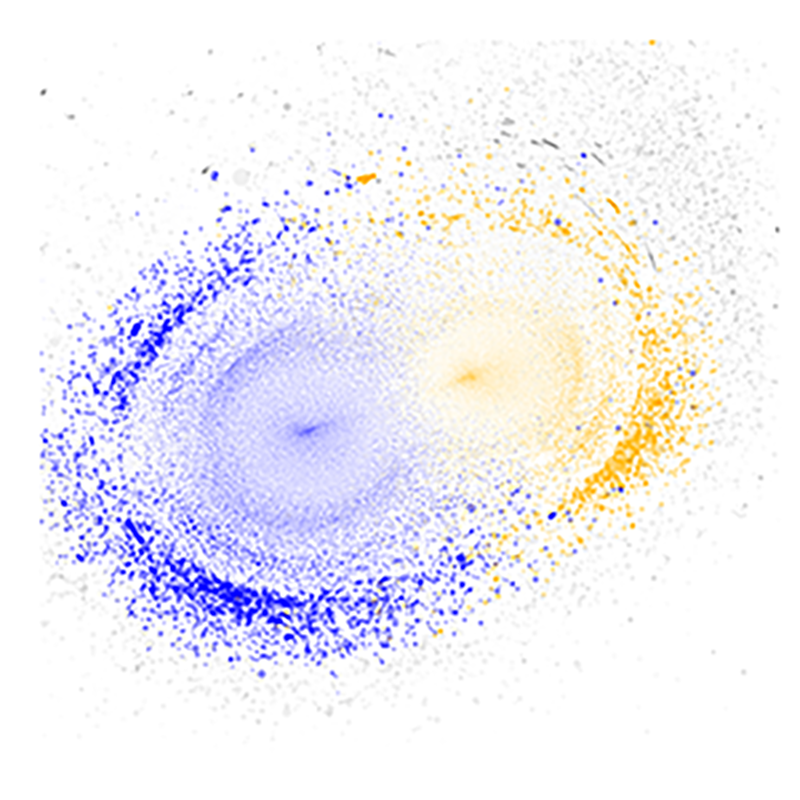
\includegraphics[width=.8\linewidth]{net_red}
\caption{Placeholder image of a Network with a long example caption to show justification setting.}
\label{fig:net}
\end{figure}


Figure \ref{fig:net} shows an example of how to insert a column-wide figure. To insert a figure wider than one column, please use the \verb|\begin{figure*}...\end{figure*}| environment. Figures wider than one column should be sized to 11.4 cm or 17.8 cm wide. Use \verb|\begin{SCfigure*}...\end{SCfigure*}| for a wide figure with side captions.





\begin{table}%[tbhp]
	%\centering
	\caption{Character Level Combat Outcomes\label{table:char_main}}
	\begin{tabular}{@{\extracolsep{5pt}}lccc} 
		\\[-1.8ex]\hline 
		\hline \\[-1.8ex] 
		& \multicolumn{3}{c}{\textit{Dependent variable:}} \\ 
		\cline{2-4} 
		\\[-1.8ex] & Combat & Combat & Combat\\ 
		\\[-1.8ex] & Amount & Variability & Skill \\ 
		\\[-1.8ex] & (1) & (2) & (3)\\ 
		\hline \\[-1.8ex] 
		Man - Male & 0.042$^{***}$ & 5.659$^{***}$ & 0.031$^{***}$  \\ 
		& (0.002) & (0.056) & (0.0004)  \\ 
		Woman - Female & $-$0.026$^{***}$ & 1.529$^{***}$ & 0.011$^{***}$  \\ 
		& (0.005) & (0.143) & (0.001)  \\ 
		Woman - Male & 0.010 & 0.375 & 0.005$^{*}$  \\ 
		& (0.009) & (0.272) & (0.002)  \\ 
		Player Age & $-$0.077$^{***}$ &  &  $-$0.003$^{***}$\\ 
		& (0.001) &  & (0.0002) \\ 
		Mil. Label & 0.135$^{***}$ &  & 0.060$^{***}$ \\ 
		& (0.002) &  & (0.0004) \\ 
		Constant &  & $-$97.425$^{***}$ &   \\ 
		&  & (0.046) &   \\ 
		\hline 
		Char. Order FEs     &       Y&       N&     Y\\
		Create Date FEs     &       Y&       N&     Y\\
		\hline  
		Observations & 576,430 & 576,430 & 576,430 \\ 
		R$^{2}$ & 0.028 & 0.018 & 0.089  \\ 
		\hline 
	\end{tabular} 
	\vspace{1mm}
	\addtabletext{*  p$<$0.05, ** p$<$0.01, *** p$<$0.001 \\
		This table reports coefficients and standards errors from ordinary least squares regressions. In all models we can reject the null that \emph{Woman - Female} and \emph{Woman - Male} are equivalent with p $<$ .01. In models 2 and 3 we can reject the null that the gender gaps within sex are equivalent ((\emph{Woman - Male}) - (\emph{Woman - Female}) = \emph{Man - Male}) with p $<$ .001.}
\end{table}


\subsection*{Tables}
In addition to including your tables within this manuscript file, PNAS requires that each table be uploaded to the submission separately as a “Table” file.  Please ensure that each table .tex file contains a preamble, the \verb|\begin{document}| command, and the \verb|\end{document}| command. This is necessary so that the submission system can convert each file to PDF.

\subsection*{Equations}

Authors may use 1- or 2-column equations in their article, according to their preference.

To allow an equation to span both columns, use the \verb|\begin{figure*}...\end{figure*}| environment mentioned above for figures. Using only \verb|\begin{figure*}...\end{figure*}| keeps the equation in a two collum format


\begin{figure}[bt!]
\begin{align*}
(x+y)^3&=(x+y)(x+y)^2\\
       &=(x+y)(x^2+2xy+y^2) \numberthis \label{eqn:example} \\
       &=x^3+3x^2y+3xy^3+x^3. 
\end{align*}
\end{figure}


\section*{References}

References should be cited in alphabethical order; this will be done automatically via bibtex, e.g. \cite{Calvo2015}, 
and \cite{Birnir2018}. All references should be included in the main manuscript file.  


\acknow{Please include your acknowledgments here, set in a single paragraph. Please do not include any acknowledgments in the Supporting Information, or anywhere else in the manuscript.}

\showacknow{} % Display the acknowledgments section

% Bibliography

\bibliography{ilcss-sample}

\end{document}